\documentclass{article}
\usepackage[utf8]{inputenc}
\usepackage[spanish]{babel}
\usepackage{graphicx}
\usepackage{anysize}
\usepackage{fancyhdr} 
\usepackage[export]{adjustbox}
\usepackage{titlesec}
\usepackage{enumitem}

% \usepackage{hyperref}
% \usepackage{float}
% \usepackage{tabu}

% Izquierda, derecha, arriba, abajo
\marginsize{2cm}{2cm}{1.2cm}{1cm} 
\renewcommand{\familydefault}{\sfdefault}
\decimalpoint%

\graphicspath{{assets/}{bdd_prac_03.assets/}}

\setlength{\parindent}{0in}
\titleformat*{\section}{\large\bfseries}

\newcommand{\materia}{BDD}
\newcommand{\clave}{2947}
\newcommand{\profesor}{Ing. Rodriguez Campos \textsc{Jorge Alberto}}
\newcommand{\grupo}{1}
\newcommand{\semestre}{2021-1}

\newcommand{\alumno}{Francisco Pablo \textsc{Rodrigo}}

\newcommand{\actividad}{Práctica 03}
\newcommand{\titulo}{Creación de una base de datos con Oracle 18c}

\newcommand{\fechaEntrega}{15 de octubre de 2020}

%%%%%%%%%%%%%%%%%%%% ENCABEZADO %%%%%%%%%%%%%%%%%%%%%%%%%%%%
\pagestyle{fancy}
\fancyhf{}
\renewcommand{\headrulewidth}{0pt}
\fancyhead[R]{% Left header
    \begin{tabular}{l}
        \materia \\ 
        \actividad%
    \end{tabular}
    \,% Space
    \rule[-1.75\baselineskip]{0pt}{0pt}
    % Strut to ensure a 1/4 \baselineskip between image and header rule
    
\includegraphics[height=3\baselineskip,valign=c]{unam}
}
\setlength{\headsep}{0.3in}


\begin{document}
%%%%%%%%%%%%%%%%%%% DATOS PORTADA %%%%%%%%%%%%%%%%%%%%%%%%
\thispagestyle{empty}
\begin{minipage}[t][5cm][t]{0.2\linewidth}
    
\includegraphics[width=2.5cm]{unam.jpg}
    \vspace{10cm}

    
\includegraphics[width=2.5cm]{fiblack}
\end{minipage}
\begin{minipage}[t]{0.7\linewidth}
    \vspace{-2.5cm}
    \LARGE{\textbf{Universidad Nacional Autónoma de México}}\\
    \Large{\textbf{Facultad de Ingeniería}} \\

    \large{\semestre}\\[2cm]

    \large{\textbf{\materia (\clave)}}\\
    \large{\textbf{Gpo: 1}}\\[5mm]
    \large{\textbf{Profesor:} \profesor}\\ [1.5cm]
    \begin{center}
        \LARGE{\textbf{\actividad}}\\
        \LARGE{\textbf{\titulo}}\\
    \end{center}

    \vspace{3.3cm}

    \large{\textbf{Alumno:} \alumno} \\[1.5cm]

    \begin{flushright}
        \fechaEntrega%
    \end{flushright}
\end{minipage}

\newpage
%%%%%%%%%%%%%%%%%%% CONTENIDO %%%%%%%%%%%%%%%%%%%%%%%%

\section*{Introducción}
% TODO:- Hacer introducción en tiempo futuro
En está práctica se analizará la instalación de una base de datos utilizando 
la arquitectura \textit{multitenant} de Oracle. Dicha arquitectura se basa en 
tener un \textit{contenedor} (root container, CDB) con varias bases de datos
inquilinas llamadas \textit{pluggable databases} (PDBs), cuya caracteristica 
principal es que pueden asociarse o desasociarse de un CDB sin tener que 
modificar los esquemas y/o objetos que contiene cada PDB.\\

Cabe destacar que para esta configuración se requiere un espacio de 
almacenamiento de entre 5 a 7 GB (solo para dos PDBs), de lo contrario no 
funcionará a menos que mandemos la instalación a una partición con mayor 
espacio disponible.\\ 

Por último, está arquictetura nos permitirá simular una arquitectura de base
de datos distribuida ya que la manera real sería costosa de implementar pues 
se requieren de por lo menos dos laptops, cada una con por los menos dos 
medios de almacenamiento.

\section*{Objetivos}
Conocer y poner en práctica las actividades requeridas para crear una base de 
datos en Oracle. Comprender y poner en práctica los conceptos básicos de la 
arquitectura Multitenant de Oracle 18c la cual será empleada en prácticas 
posteriores para ``simular'' una BDD.

% \section*{Desarrollo}
\section*{C1. Pantalla que muestra que la instancia y
el listener están detenidos.}

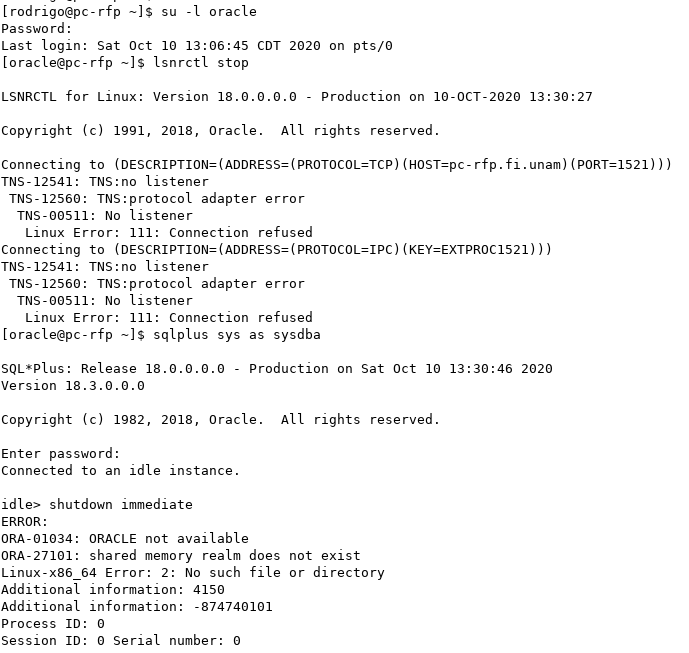
\includegraphics[width=0.8\linewidth]{c1}

\section*{C2. Pantalla que muestra el listener
iniciado, instancia detenida.}

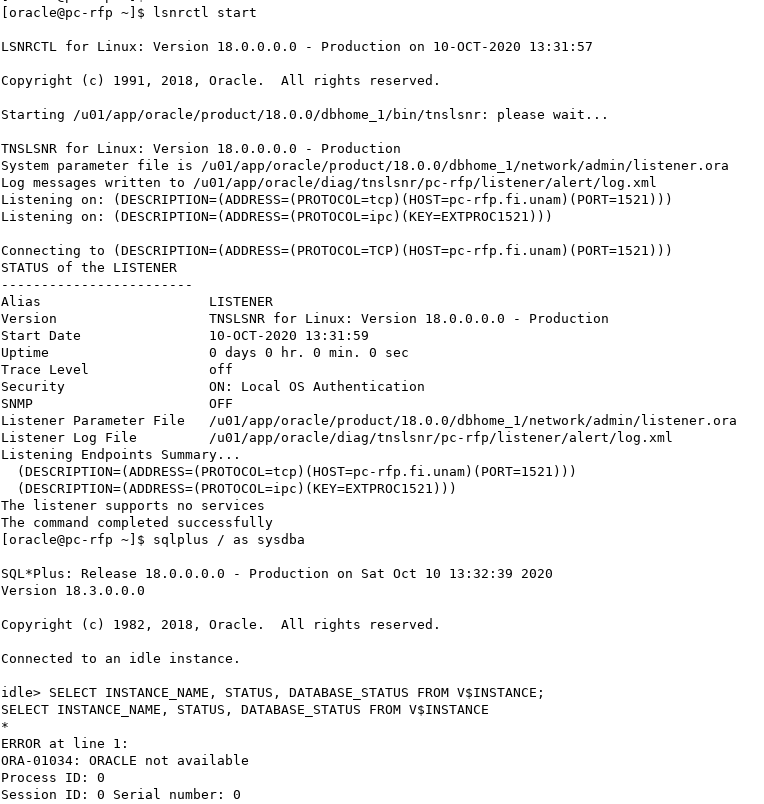
\includegraphics[width=0.8\linewidth]{c2}

\section*{C3. Pantalla que muestra listener e
instancia listos para recibir peticiones.}

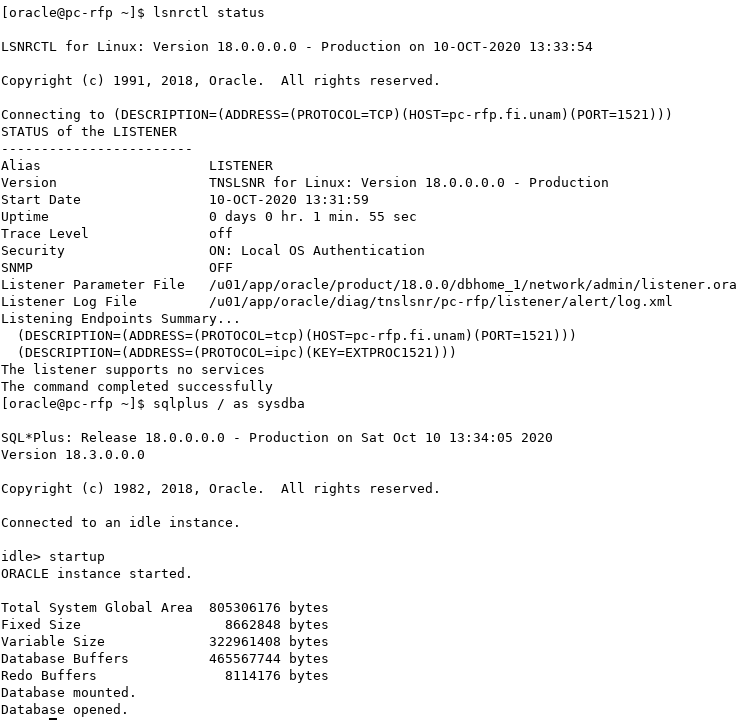
\includegraphics[width=0.8\linewidth]{c3}

\section*{C4. Diferencias encontradas en las 3
consultas del punto anterior.}

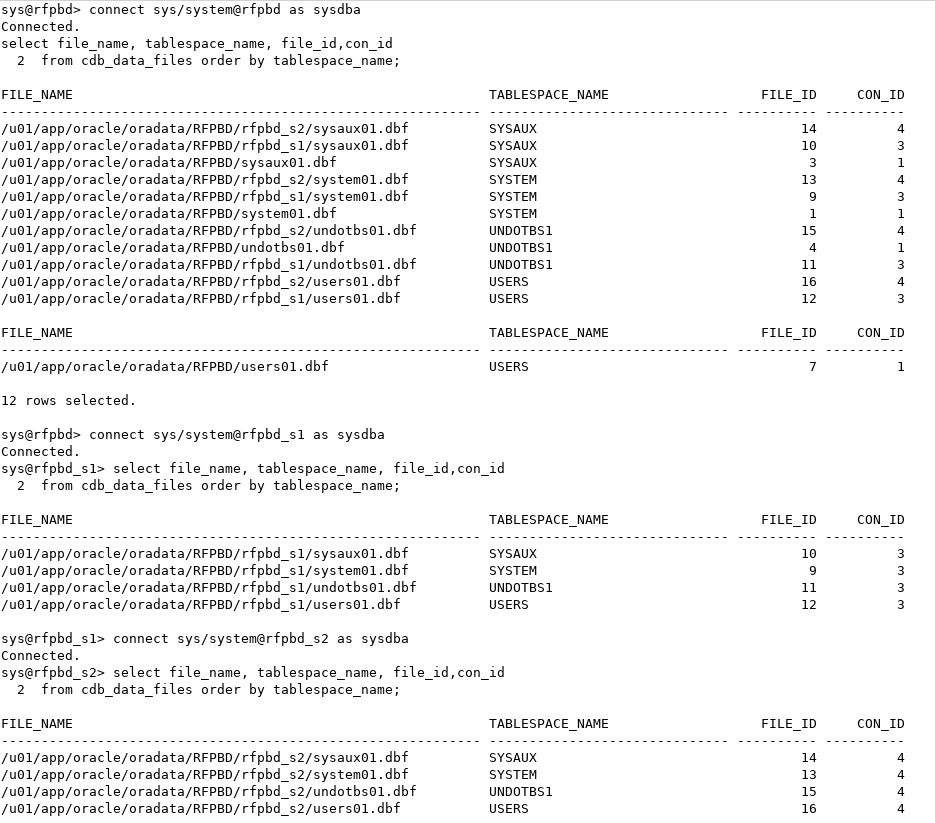
\includegraphics[width=\linewidth]{c4}\\

En la imagen se observa que la principal diferencia radica en los 
\textit{file names} a los que tiene acceso.
\begin{itemize}
    \item Los \textbf{PDBs} solos tienen acceso a sus database files,
    \item por otra parte, el \textbf{Root Container} o simplemente contenedor
    tiene acceso los database files de los PDBs y algunos otros archivos.
\end{itemize}

\section*{C5. Salida del script de validación}

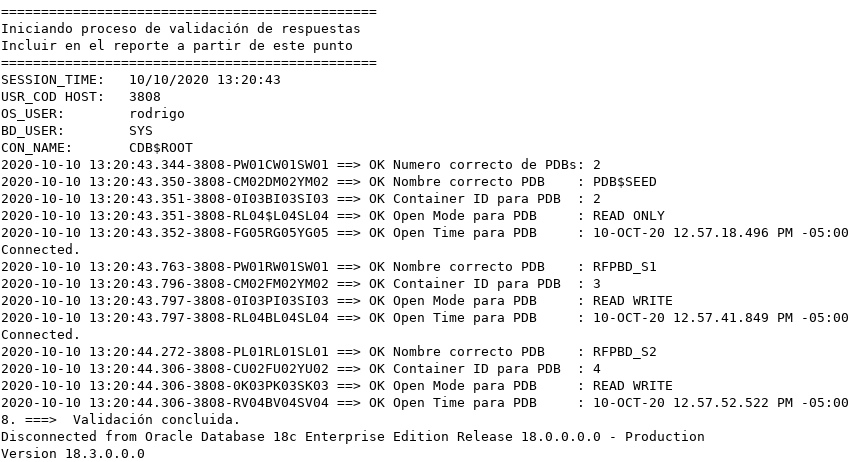
\includegraphics[width=0.9\linewidth]{c5}

\section*{Comentarios y conclusiones}

La instalación de una \textit{base de datos multitenant} resulta 
un procedimiento bastante sencillo gracias al \textit{dbca}, de hecho, es 
prácticamente la misma instalación que una base de datos normal, con la 
excepción de que debemos de elegir la opción de crear un contenedor y elegir 
el número de PDBs.\\

Por otra parte, me atrevo a decir que esta arquitectura es frecuentemente 
utiliza en la industria y debido a eso es que Oracle casi todo preparado
para que la instalación se haga de manera sencilla, de hecho la casilla de 
\textit{crear contenedor} viene marcada por defecto.\\

Por último, el concepto de \textit{pluggable databases} se me hizo muy 
interesante porque permite hacer más flexible nuestra base de datos y agregar 
una capa extra de organización (además de la de los usuarios), lo cual
podría ser bastante útil para tener un mayor grado de seguridad y mantenimiento.

\renewcommand\refname{Bibliografía}
\begin{thebibliography}{99}
    \bibitem{oracle} Oracle. \textit{Oracle Database Documentation} en 
        \texttt{https://docs.oracle.com/en/database/oracle/\\oracle-database/%
        index.html}
\end{thebibliography}

\end{document}
